\providecommand{\Cart}{\mathcal{C}art}
\providecommand{\coCart}{\mathrm{co}\mathcal{C}\mathit{art}}   %
\providecommand{\Fib}{\mathcal{F}ib}
\providecommand{\Mod}{\mathrm{Mod}}
\providecommand{\Fun}{\operatorname{Fun}}
\providecommand{\qcor}[1]{\ulcorner#1\urcorner}   %


\begin{proposition}[双侧纤维化的单侧 \trYonedaLemma]\label{prop:one-sided-yoneda-two-sided}
对任意\trFunctor{} $f\colon A\to B$ 与\trTwoSidedIsofibration{}
$A\xleftarrow{q}E\xrightarrow{p}B$，沿
$\qcor{\mathrm{id}_{f}}\colon A\to\mathrm{Hom}_{B}(B,f)$ 作限制，诱导出%
\trQuasiCategory{}之间的一个\trEquivalence
{\small\[
\mathrm{Fun}_{A\times B}^{\mathrm{cart}}\!\left(
\begin{gathered}
\mathrm{Hom}_{B}(B,f)\\[-2pt]
\downarrow\scriptstyle (p_{1},\,p_{0})\\[-2pt]
A\times B
\end{gathered}
\;\right.,
\left.
\begin{gathered}
E\\[-2pt]
\downarrow\scriptstyle (q,\,p)\\[-2pt]
A\times B
\end{gathered}
\right)
\xrightarrow[\ \sim\ ]{\ \mathrm{ev}_{\qcor{\mathrm{id}_{f}}}\ }
\mathrm{Fun}_{A\times B}\!\left(
\begin{gathered}
A\\[-2pt]
\downarrow\scriptstyle (\mathrm{id},\,f)\\[-2pt]
A\times B
\end{gathered}
\;\right.,
\left.
\begin{gathered}
E\\[-2pt]
\downarrow\scriptstyle (q,\,p)\\[-2pt]
A\times B
\end{gathered}
\right)
\]}
\end{proposition}

\begin{proof}
这只需对元素 $(\mathrm{id},f)\colon A\to A\times B$ 与\trInfinityCosmos{}
$\coCart(\mathcal{K})_{/A}$ 中的\trCartesianFibration{}
$(q,p)\colon E\twoheadrightarrow A\times B$ 应用定理 5.7.3 的\trYonedaLemma{}即得。
\end{proof}

\subsection*{练习}

\begin{exercise}\label{ex:other-one-sided-yoneda}
陈述并证明双侧纤维化的另一个单侧\trYonedaLemma{}：建立由沿函子
$\qcor{\mathrm{id}_{f}}\colon B\to\mathrm{Hom}_{A}(f,A)$ 作限制所诱导的诸%
\trFunctorSpace{}之间的如下\trEquivalence
{\small\[
\mathrm{Fun}_{A\times B}^{\mathrm{cart}}\!\left(
\begin{gathered}
\mathrm{Hom}_{A}(f,A)\\[-2pt]
\downarrow\scriptstyle (p_{1},\,p_{0})\\[-2pt]
A\times B
\end{gathered}
\;\right.,
\left.
\begin{gathered}
E\\[-2pt]
\downarrow\scriptstyle (q,\,p)\\[-2pt]
A\times B
\end{gathered}
\right)
\xrightarrow{\ \sim\ }
\mathrm{Fun}_{A\times B}\!\left(
\begin{gathered}
B\\[-2pt]
\downarrow\scriptstyle (f,\,\mathrm{id})\\[-2pt]
A\times B
\end{gathered}
\;\right.,
\left.
\begin{gathered}
E\\[-2pt]
\downarrow\scriptstyle (q,\,p)\\[-2pt]
A\times B
\end{gathered}
\right)
\]}
\end{exercise}

\section{作为离散双侧纤维化的模}\label{sec:modules-as-discrete-two-sided-fibrations}

现在我们将注意力转向某些\trTwoSidedFibration{}的特殊性质；诸如逗号\trSpan{}这样的%
\trTwoSidedFibration{}，作为\trSliceInfinityCosmos{}中的对象是\trDiscrete{}。

\begin{definition}\label{def:modules}
\trInfinityCosmos{} $\mathcal{K}$ 中从 $A$ 到 $B$ 的一个\textbf{\trModule}%
（module）是一条\trTwoSidedFibration{}
$A\overset{q}{\twoheadleftarrow}E\overset{p}{\twoheadrightarrow}B$，它在
${}_{A\backslash}\Fib(\mathcal{K})_{/B}$ 中是一个\trDiscrete{}对象。
\end{definition}

\trCosmologicallyEmbedded{}\trInfinityCosmos{}
${}_{A\backslash}\Fib(\mathcal{K})_{/B}\hookrightarrow\mathcal{K}_{/A\times B}$
中的一个对象在其中是\trDiscrete{}，当且仅当它作为 $\mathcal{K}_{/A\times B}$
的对象是\trDiscrete{}（见练习 6.3.iv）。我们在此章中的工作使我们得以给出%
\trModule{}的一个直接刻画：

\begin{proposition}\label{prop:module-characterization}
一个\trTwoSidedIsofibration{} $A\xleftarrow{q}E\xrightarrow{p}B$ 定义一个从
$A$ 到 $B$
的\trModule{}，当且仅当它
\begin{enumerate}[label=(\roman*)]
\item 左侧余笛卡尔，
\item 右侧笛卡尔，
\item 并且作为 $\mathcal{K}_{/A\times B}$ 的对象是\trDiscrete{}。
\end{enumerate}
\end{proposition}

\begin{proof}
把\cref{def:modules}与本陈述相比较，可见我们只需论证：这三条性质足以证明 $E$
是一个从 $A$ 到 $B$ 的\trTwoSidedFibration{}。定理 7.1.4(iv) 告诉我们：%
\trInfinityCosmos{} $\mathcal{K}$ 中一个从 $A$ 到 $B$ 的\trTwoSidedFibration{}
$E$ 是一条\trTwoSidedIsofibration{}，它左侧余笛卡尔、右侧笛卡尔，并且使 $\mathcal{K}_{/A\times B}$
中某一支以 $E$ 为余定义域的\trNaturalTransformation{}为一个\trIsomorphism{}。当
$E$ 是 $\mathcal{K}_{/A\times B}$ 中的\trDiscrete{}对象时，以 $E$ 为余定义域的
一切\trNaturalTransformation{}都可逆，故性质 (i)、(ii) 与 (iii) 已足够。
\end{proof}

\trModule{}的下述诸性质可以很容易地从我们关于\trTwoSidedFibration{}的结果中
推导出来。

\begin{lemma}\label{lem:module-properties}
若 $A\overset{q}{\twoheadleftarrow}E\overset{p}{\twoheadrightarrow}B$ 在%
\trInfinityCosmos{} $\mathcal{K}$ 中定义一个从 $A$ 到 $B$ 的\trModule{}，则
\begin{enumerate}[label=(\roman*)]
\item 下式所示的诸\trFunctor{}分别在\trInfinityCosmos{}
$\Cart(\mathcal{K})_{/B}$ 与 $\coCart(\mathcal{K})_{/A}$ 中定义一条离散%
\trCocartesianFibration{}与一条离散\trCartesianFibration{}。
\begin{center}
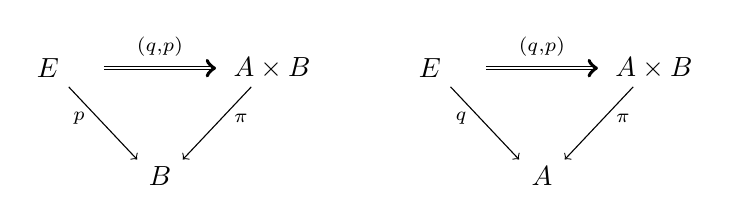
\begin{tikzpicture}[x=1.5em,y=1.5em]
  \begin{scope}[shift={(0,0)}]
  \node (E)  at (0,1.3) {$E$};
  \node (AB) at (5.4,1.3) {$A\times B$};
  \node (B)  at (2.7,-1.3) {$B$};
  \draw[double,->] (1.35,1.3) -- (4.05,1.3);
  \node at (2.7,1.82) {$\scriptstyle(q,p)$};
  \draw[->] (0.5,0.85) -- (2.15,-0.9);
  \node at (0.75,0.1) {$\scriptstyle p$};
  \draw[->] (4.9,0.85) -- (3.25,-0.9);
  \node at (4.65,0.1) {$\scriptstyle\pi$};
  \end{scope}
  \begin{scope}[shift={(9.2,0)}]
  \node (E)  at (0,1.3) {$E$};
  \node (AB) at (5.4,1.3) {$A\times B$};
  \node (A)  at (2.7,-1.3) {$A$};
  \draw[double,->] (1.35,1.3) -- (4.05,1.3);
  \node at (2.7,1.82) {$\scriptstyle(q,p)$};
  \draw[->] (0.5,0.85) -- (2.15,-0.9);
  \node at (0.75,0.1) {$\scriptstyle q$};
  \draw[->] (4.9,0.85) -- (3.25,-0.9);
  \node at (4.65,0.1) {$\scriptstyle\pi$};
  \end{scope}
\end{tikzpicture}
\end{center}
\item 诸\trFunctor{} $q\colon E\twoheadrightarrow A$ 与
$p\colon E\twoheadrightarrow B$ 分别在 $\mathcal{K}$ 中定义一条%
\trCocartesianFibration{}与一条\trCartesianFibration{}。
\item 对任意以 $E$ 为余定义域的\trNaturalTransformation{} $\psi$，$\psi$ 是
$p$-笛卡尔的当且仅当 $q\psi$ 可逆，而 $\psi$ 是 $q$-余笛卡尔的当且仅当
$p\psi$ 可逆。
\item 特别地，在 $A\times B$ 之上纤维化的任何\trNaturalTransformation{}既是
$p$-笛卡尔的又是 $q$-余笛卡尔的，\footnote{原书印作「is both $p$- and
$q$-cocartesian」，按条件 (iii) 应为「既是 $p$-笛卡尔的又是 $q$-余笛卡尔的」，
疑原书脱「cartesian」字，此处径改。——译者注}并且从如下所示的双侧纤维化
\begin{center}
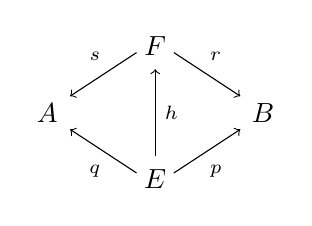
\begin{tikzpicture}[x=1.5em,y=1.5em]
  \node (F) at (2.6,1.6) {$F$};
  \node (A) at (0,0) {$A$};
  \node (B) at (5.2,0) {$B$};
  \node (E) at (2.6,-1.6) {$E$};
  \draw[->] (2.15,1.45) -- node[above left,pos=0.4]{$\scriptstyle s$} (0.55,0.4);
  \draw[->] (3.05,1.45) -- node[above right,pos=0.4]{$\scriptstyle r$} (4.65,0.4);
  \draw[->] (2.6,-1.05) -- node[right,pos=0.5]{$\scriptstyle h$} (2.6,1.05);
  \draw[->] (2.15,-1.45) -- node[below left,pos=0.4]{$\scriptstyle q$} (0.55,-0.4);
  \draw[->] (3.05,-1.45) -- node[below right,pos=0.4]{$\scriptstyle p$} (4.65,-0.4);
\end{tikzpicture}
\end{center}
到一个\trModule{}的任何\trSpan{}映射，都定义诸\trTwoSidedFibration{}之间的一个%
\trCartesianFunctor{}，同时也定义从 $s$ 到 $q$ 与从 $r$ 到 $p$ 的\trCartesianFunctor{}。
\end{enumerate}
\end{lemma}

\begin{proof}
由引理 7.1.1，\cref{prop:module-characterization}的条件 (ii) 与 (iii) 合并起来
告诉我们：\trTwoSidedIsofibration{} $(q,p)\colon E\twoheadrightarrow A\times B$ 在
$\mathcal{K}_{/A}$ 中定义一条离散\trCartesianFibration{}。由于\trModule{}都是%
\trTwoSidedFibration{}，而离散性被\trCosmologicalEmbedding{}所反射，事实上
$(q,p)\colon E\twoheadrightarrow A\times B$ 在 $\coCart(\mathcal{K})_{/A}$ 中
定义一条离散\trCartesianFibration{}，这就证明了 (i)。

陈述 (ii) 对任何\trTwoSidedFibration{}都成立（见引理 7.1.1(iv)）。在此重申它的
要点在于强调：\trModule{}的两条腿本身未必是离散\trFibration{}（见%
\cref{ex:module-legs-not-discrete}）。

陈述 (iii) 的一个方向已作为引理 7.1.1(iv) 证得。对于其逆向，考虑某一以 $E$ 为
余定义域的\trNaturalTransformation{} $\psi$，并设 $q\psi$ 可逆。与 $q\psi^{-1}$
沿\trIsofibration{} $q\colon E\twoheadrightarrow A$ 的一个提升作复合后，便可见 $\psi$
同构于使 $q\psi'$ 为恒同的一个\trNaturalTransformation{} $\psi'$。由 $p$-笛卡尔
变换的同构稳定性，只需证明 $\psi'$ 是 $p$-笛卡尔的。由命题 3.6.2，$\psi'$ 可以
沿覆盖 2-函子 $\mathfrak{h}(\mathcal{K}_{/A})\to(\mathfrak{h}\mathcal{K})_{/A}$
提升为\trSliceInfinityCosmos{} $\mathcal{K}_{/A}$ 中一支以
$q\colon E\twoheadrightarrow A$ 为余定义域的\trNaturalTransformation{}；由于
通常施行这类提升而不加评注，我们对 $\mathcal{K}_{/A}$ 中的纤维化%
\trNaturalTransformation{}保留记号 $\psi'$。由于
$(q,p)\colon E\twoheadrightarrow A\times B$ 是 $\mathcal{K}_{/A}$ 中的一条离散%
\trCartesianFibration{}，每一支此类\trNaturalTransformation{}都是
$(q,p)$-笛卡尔的。由定理 5.2.8(iii)，由此推知 $\psi'$ 同构于 $A\times B$ 之上的%
\trFiberedAdjunction{} $\Delta_{p}\dashv r$ 的\trCounit{}的某支须化副本。由于同一份数据——
此次视为 $B$ 之上的一个\trFiberedAdjunction——见证了 $p\colon E\twoheadrightarrow B$ 是
一条\trCartesianFibration{}这一事实，定理 5.2.8(iii) 便也告诉我们：$\psi'$
从而 $\psi$ 是 $p$-笛卡尔的，恰如所断言。

陈述 (iv) 由 (iii) 与命题 7.1.7(iv) 推得。
\end{proof}

由于诸\trModule{}恰好是\trTwoSidedFibration{}的\trInfinityCosmos{}中的%
\trDiscrete{}对象：

\begin{corollary}\label{cor:module-cosmos}
对\trInfinityCosmos{} $\mathcal{K}$ 中任意一对\trInfinityCategory{} $A$ 与
$B$，存在一个\trCosmologicallyEmbedded{}\trInfinityCosmos
\begin{center}
\begin{tikzpicture}[x=1.5em,y=1.5em]
  \node (Mod) at (0,1.5) {${}_{A\backslash}\Mod(\mathcal{K})_{/B}$};
  \node (Fib) at (10.6,1.5) {${}_{A\backslash}\Fib(\mathcal{K})_{/B}$};
  \node (K)   at (5.3,-1.4) {$\mathcal{K}_{/A\times B}$};
  \draw[right hook->] (3.0,1.5) -- (7.6,1.5);
  \draw[right hook->] (0.45,0.95) -- (3.95,-0.8);
  \draw[right hook->] (10.15,0.95) -- (6.65,-0.8);
\end{tikzpicture}
\end{center}
它定义为从 $A$ 到 $B$ 的\trTwoSidedFibration{}的\trInfinityCosmos{}或从 $A$ 到
$B$ 的\trIsofibration{}的\trInfinityCosmos{}中的一个全子范畴。
\end{corollary}

\begin{proof}
命题 6.1.6 证明了
${}_{A\backslash}\Mod(\mathcal{K})_{/B}\hookrightarrow{}_{A\backslash}\Fib(\mathcal{K})_{/B}$
是命题 7.2.2 的\trInfinityCosmos{}中一个\trCosmologicallyEmbedded{}子∞-宇宙，
而\cref{lem:module-properties}(iv)
证明了包含
${}_{A\backslash}\Mod(\mathcal{K})_{/B}\hookrightarrow\mathcal{K}_{/A\times B}$
也是满的。
\end{proof}

\trModule{}的一个重要性质是它在\trPullback{}之下稳定：

\begin{proposition}\label{prop:module-pullback}
若 $A\twoheadleftarrow E\twoheadrightarrow B$ 是一个从
$A$ 到 $B$ 的\trModule{}，而 $a\colon A'\to A$ 与 $b\colon B'\to B$ 是任意一对%
\trFunctor{}，则该\trPullback{}定义一个从 $A'$ 到 $B'$ 的\trModule
$A'\twoheadleftarrow E(b,a)\twoheadrightarrow B'$
\begin{center}
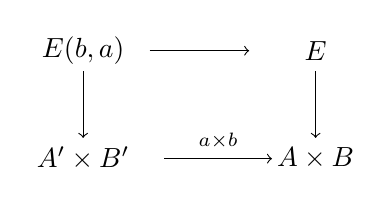
\begin{tikzpicture}[x=1.5em,y=1.5em]
  \node (Eba) at (0,1.3) {$E(b,a)$};
  \node (E)   at (5.6,1.3) {$E$};
  \node (ABp) at (0,-1.3) {$A'\times B'$};
  \node (AB)  at (5.6,-1.3) {$A\times B$};
  \draw[->] (1.6,1.3) -- (4.0,1.3);
  \draw[->] (0,0.8) -- (0,-0.8);
  \draw[->] (5.6,0.8) -- (5.6,-0.8);
  \draw[->] (1.95,-1.3) -- node[above]{$\scriptstyle a\times b$} (4.55,-1.3);
  \node at (0.8,0.5) {$\scriptstyle\lrcorner$};
\end{tikzpicture}
\end{center}
\end{proposition}

\begin{proof}
命题 7.2.4 的\trCosmologicalFunctor
$(a,b)^{*}\colon{}_{A\backslash}\Fib(\mathcal{K})_{/B}\to{}_{A'\backslash}\Fib(\mathcal{K})_{/B'}$
与一切\trCosmologicalFunctor{}一样，保持\trDiscrete{}对象。
\end{proof}

把\cref{prop:module-pullback}应用于一对元素 $a\colon 1\to A$ 与
$b\colon 1\to B$，便可见一个从 $A$ 到 $B$ 的\trModule{}是一条%
\trTwoSidedFibration{}，其诸\trFiber{} $E(b,a)$ 都是\trDiscrete{}%
\trInfinityCategory{}。其逆一般并不成立，因为作为\trSliceInfinityCosmos{}
$\mathcal{K}_{/A\times B}$ 的对象是\trDiscrete{}，这一条件比仅仅具有离散%
\trFiber{}更强。然而，当 $\mathcal{K}$ 是一个由 $(\infty,1)$-范畴构成的%
\trInfinityCosmos{}时，命题 12.2.3 证明：切片中的离散性由逐纤维离散性推得。

\trModule{}的原型例由\trArrowInfinityCategory{}构造与\trCommaInfinityCategory{}%
构造给出。

\begin{proposition}[逗号∞-范畴都是模]\label{prop:comma-infinity-categories-are-modules}
\begin{enumerate}[label=(\roman*)]
\item 对任意\trInfinityCategory{} $A$，\trArrowInfinityCategory{} $A^{2}$ 定义
一个从 $A$ 到 $A$ 的\trModule{}。
\item 对任意\trCospan{} $C\overset{g}{\rightarrow}A\overset{f}{\leftarrow}B$，
\trCommaInfinityCategory{} $\mathrm{Hom}_{A}(f,g)$ 定义一个从 $C$ 到 $B$ 的%
\trModule{}。
\end{enumerate}
\end{proposition}

正如刚才所评注的，$A^{2}\twoheadrightarrow A\times A$ 是离散的这一事实，与命题
3.4.10 所证明的那桩事实——$A$ 的任意一对元素之间的\trMappingSpace{}是一个%
\trDiscrete{}\trInfinityCategory——相关联，但比后者更强。

\begin{proof}
由\cref{prop:module-pullback}，第二条陈述可以由第一条推得；不过，用我们这一整套
既有结果来一举证明两条陈述并不更难。命题 7.1.6 与例 7.2.8 证明了箭头\trSpan{}与
逗号\trSpan{}定义\trTwoSidedFibration{}，故尚待验证的只有离散性条件。由引理
5.5.1，$A^{2}\twoheadrightarrow A\times A$ 在 $A\times A$ 之上的%
\trSliceInfinityCosmos{}中的离散性、以及
$\mathrm{Hom}_{A}(f,g)\twoheadrightarrow C\times B$ 在 $C\times B$ 之上的%
\trSliceInfinityCosmos{}中的离散性，都是命题 3.2.5 与命题 3.4.6 的%
\trTwoCellConservativity{}的直接推论：就后者而言，若 $\tau$ 是任意一支以
$\mathrm{Hom}_{A}(f,g)$ 为余定义域的\trCell{}，使得 $p_{1}\tau$ 与 $p_{0}\tau$
可逆，则 $\tau$ 本身可逆。
\end{proof}

这些\trCommaModule{}的两个特例——即 3.5 节中所研究的那些——值得专门命名：

\begin{definition}\label{def:represented-modules}
对\trInfinityCategory{}之间的任意\trFunctor{} $f\colon A\to B$，
\begin{enumerate}[label=(\roman*)]
\item 从 $A$ 到 $B$ 的\trModule{} $\mathrm{Hom}_{B}(B,f)$ 称为被 $f$
\textbf{右表示}（right represented）或\textbf{协变表示}（covariantly
represented），
\item 而从 $B$ 到 $A$ 的\trModule{} $\mathrm{Hom}_{B}(f,B)$ 称为被 $f$
\textbf{左表示}（left represented）或\textbf{反变表示}（contravariantly
represented）。
\end{enumerate}
更一般地，若一个\trModule{}与左表示或右表示的诸模\trFiberedEquivalence{}，则称它
被 $f$ \textbf{协变表示}或\textbf{反变表示}。
\end{definition}

如 5.7 节中那样，当映入一个\trModule{}时，双侧纤维化的\trYonedaLemma{}便会
简化，其原因在于\cref{lem:module-properties}(iv) 的观察：从一支%
\trTwoSidedFibration{}到一个\trModule{}的任何\trSpan{}映射都定义一个%
\trCartesianFunctor{}。

\begin{theorem}[模的 \trYonedaLemma]\label{thm:yoneda-for-modules}
对任意\trSpan{} $A\overset{a}{\leftarrow}X\overset{b}{\rightarrow}B$ 与任意%
\trModule{}
$A\overset{q}{\twoheadleftarrow}E\overset{p}{\twoheadrightarrow}B$，沿
$(\qcor{\mathrm{id}_{a}},\qcor{\mathrm{id}_{b}})\colon X\to\mathrm{Hom}_{A}(a,A)\times_{X}\mathrm{Hom}_{B}(B,b)$ 作限制定义了%
\trKanComplex{}之间的一个\trEquivalence
{\small\[
\mathrm{Fun}_{A\times B}\!\left(
\begin{gathered}
\mathrm{Hom}_{A}(a,A)\times_{X}\mathrm{Hom}_{B}(B,b)\\[-2pt]
\downarrow\scriptstyle (p_{1}\pi_{1},\,p_{0}\pi_{0})\\[-2pt]
A\times B
\end{gathered}
\;\right.,
\left.
\begin{gathered}
E\\[-2pt]
\downarrow\scriptstyle (q,\,p)\\[-2pt]
A\times B
\end{gathered}
\right)
\xrightarrow[\ \sim\ ]{\ \mathrm{ev}_{(\qcor{\mathrm{id}_{a}},\,\qcor{\mathrm{id}_{b}})}\ }
\mathrm{Fun}_{A\times B}\!\left(
\begin{gathered}
X\\[-2pt]
\downarrow\scriptstyle (a,\,b)\\[-2pt]
A\times B
\end{gathered}
\;\right.,
\left.
\begin{gathered}
E\\[-2pt]
\downarrow\scriptstyle (q,\,p)\\[-2pt]
A\times B
\end{gathered}
\right)
\]}
而对任意\trFunctor{} $f\colon A\to B$ 或 $g\colon B\to A$，沿
$\qcor{\mathrm{id}_{f}}\colon A\to\mathrm{Hom}_{B}(B,f)$ 或
$\qcor{\mathrm{id}_{g}}\colon B\to\mathrm{Hom}_{A}(g,A)$ 作限制定义了%
\trKanComplex{}之间的诸\trEquivalence
{\small\[
\mathrm{Fun}_{A\times B}\!\left(
\begin{gathered}
\mathrm{Hom}_{B}(B,f)\\[-2pt]
\downarrow\scriptstyle (p_{1},\,p_{0})\\[-2pt]
A\times B
\end{gathered}
\;\right.,
\left.
\begin{gathered}
E\\[-2pt]
\downarrow\scriptstyle (q,\,p)\\[-2pt]
A\times B
\end{gathered}
\right)
\xrightarrow[\ \sim\ ]{\ \mathrm{ev}_{\qcor{\mathrm{id}_{f}}}\ }
\mathrm{Fun}_{A\times B}\!\left(
\begin{gathered}
A\\[-2pt]
\downarrow\scriptstyle (\mathrm{id},\,f)\\[-2pt]
A\times B
\end{gathered}
\;\right.,
\left.
\begin{gathered}
E\\[-2pt]
\downarrow\scriptstyle (q,\,p)\\[-2pt]
A\times B
\end{gathered}
\right)
\]}
{\small\[
\mathrm{Fun}_{A\times B}\!\left(
\begin{gathered}
\mathrm{Hom}_{A}(g,A)\\[-2pt]
\downarrow\scriptstyle (p_{1},\,p_{0})\\[-2pt]
A\times B
\end{gathered}
\;\right.,
\left.
\begin{gathered}
E\\[-2pt]
\downarrow\scriptstyle (q,\,p)\\[-2pt]
A\times B
\end{gathered}
\right)
\xrightarrow[\ \sim\ ]{\ \mathrm{ev}_{\qcor{\mathrm{id}_{g}}}\ }
\mathrm{Fun}_{A\times B}\!\left(
\begin{gathered}
B\\[-2pt]
\downarrow\scriptstyle (g,\,\mathrm{id})\\[-2pt]
A\times B
\end{gathered}
\;\right.,
\left.
\begin{gathered}
E\\[-2pt]
\downarrow\scriptstyle (q,\,p)\\[-2pt]
A\times B
\end{gathered}
\right)
\]}
\end{theorem}

我们尚未解释这一奇特的术语——为什么我们把离散\trTwoSidedFibration{}称作
「模」。这个名号
意在暗示：在\trModule{}的演算与那种更为人熟悉的代数结构的演算之间，存在一种
深层结构类比——下面我们就转向这一主题。

\subsection*{练习}

\begin{exercise}\label{ex:module-legs-not-discrete}
举例说明：若 $A\overset{q}{\twoheadleftarrow}E\overset{p}{\twoheadrightarrow}B$
定义一个从 $A$ 到 $B$ 的\trModule{}，则未必有 $p\colon E\twoheadrightarrow B$ 是
一条离散\trCartesianFibration{}或 $q\colon E\twoheadrightarrow A$ 是一条离散%
\trCocartesianFibration{}。
\end{exercise}

\begin{exercise}\label{ex:horizontal-composite-not-module}
\begin{enumerate}[label=(\roman*)]
\item 解释为什么命题 7.1.6 的\trTwoSidedFibration{}
$(p_{n-1},p_{0})\colon A^{\mathbb{n}}\twoheadrightarrow A\times A$ 在 $n>2$
时并不定义一个\trModule{}。
\item 由此推出：如命题 7.2.6 所定义的那般，\trModule{}的水平复合未必是一个%
\trModule{}。
\end{enumerate}
\end{exercise}

\begin{exercise}\label{ex:module-terminal-analogue}
陈述并证明练习 7.1.ii 的一个类比——刻画从 $1$ 到 $B$ 的\trModule{}与从 $B$ 到
$1$ 的\trModule——并化解这一陈述与\cref{ex:module-legs-not-discrete}之间任何
明显的冲突。
\end{exercise}

